\documentclass[UTF8,a4paper,zihao=-4]{ctexart}

\usepackage[margin=2.3cm]{geometry}
\usepackage{amsmath,amssymb}
\usepackage{booktabs}
\usepackage{array}
\usepackage{caption}
\usepackage{float}
\usepackage{graphicx}
\graphicspath{{figures/}{report/figures/}}

\pagestyle{plain}
\captionsetup{font=small,labelfont=bf}
\renewcommand{\arraystretch}{1.25}
\emergencystretch=2em

\begin{document}

\begin{titlepage}
\thispagestyle{empty}
\centering
\vspace*{2.2cm}
{\zihao{2}\bfseries 信号分离装置设计报告\par}
\vspace{0.8cm}
{\zihao{4} 作者：唐广洲\par}
\vfill
\end{titlepage}

\clearpage
\thispagestyle{plain}
\section*{摘要}
\noindent
本设计面向信号分离装置题目要求，对两路频率范围为 20 kHz--100 kHz、峰峰值为 1 V 的周期信号进行自动识别与再生。系统由独立加法器、AD7616 高速采集模块、STM32F407 主控、AD9833/AD9834 双 DDS 输出模块、后级放大模块以及 LCD 显示模块组成。输入混合信号 $C=A+B$ 经 AD7616 采样，主控完成 FFT、谱峰搜索、频率栅格吸附与波形判别，再控制 AD9833 输出低频分量 $A'$、AD9834 输出高频分量 $B'$。方案避免了固定模拟滤波器对未知频率组合的依赖，能够适应 50 kHz+100 kHz 双正弦、10 kHz 整数倍双正弦以及 5 kHz 整数倍正弦/三角波组合测试。硬件电源部分采用 TPS5430 产生正负 5 V 为 TL082 加法器运放供电，TPS5450 产生 +5 V 为 STM32F407 主控、DDS 模块及后级 OPA177 放大模块供电。
\clearpage

\setcounter{page}{1}
\let\originsection\section
\renewcommand{\section}{\clearpage\originsection}

\section{任务要求与总体指标}

题目要求制作独立加法器和分离电路。加法器实现 $C=A+B$，并且与分离电路之间除混合信号 $C$ 和地线外不得存在其他通信或控制连接。输出信号 $A'$、$B'$ 应与原信号 $A$、$B$ 同频稳定显示，波形无明显失真，峰峰值不小于 1 V。

基本要求包括 $f_A=50\text{ kHz}$、$f_B=100\text{ kHz}$ 双正弦分离，以及 $f_A$、$f_B$ 为 10 kHz 整数倍的双正弦分离。发挥部分要求 $A$、$B$ 可为正弦波或三角波，频率为 5 kHz 整数倍，并且正弦信号不落在三角波谐波分量中。

\section{方案论证与选择}

\subsection{可选方案比较}

\begin{table}[H]
\centering
\caption{信号分离方案比较}
\begin{tabular*}{\textwidth}{@{\extracolsep{\fill}}p{3.2cm}p{3.8cm}p{4.0cm}p{2.0cm}@{}}
\toprule
方案 & 优点 & 不足 & 结论 \\
\midrule
模拟滤波器组 & 电路直观，实时性好，理论成熟。 & 频率组合不固定时需要可调中心频率或大量滤波器；三角波谐波会干扰带通判断；调试量大。 & 不采用 \\
锁相/相关检测 & 对已知频率信号抗噪能力强，可估计相位。 & 需要逐频扫描或参考频率集合，频点较多时程序复杂度上升。 & 备用思路 \\
裸板采集方案 & 硬件最少，可直接使用主控片内 ADC 或简单采样电路。 & STM32F407 片内 ADC 位数和模拟前端性能有限，动态范围、同步性和抗干扰能力不足，输入保护也较弱。 & 对比方案 \\
AD9854 DDS 输出方案 & 频率分辨率高，器件能力强，适合更高频和复杂调制。 & 控制寄存器多、接口复杂，功耗和板级调试成本较高；本题只需 20--100 kHz 正弦/三角波再生，能力明显过剩。 & 不采用 \\
AD7616+F407+双 DDS & 采集分辨率高，算法灵活；AD9833/AD9834 直接产生目标波形，输出频率稳定；硬件复杂度适中。 & 依赖软件识别和 FFT 参数设计，对采样时序有要求。 & 采用 \\
\bottomrule
\end{tabular*}
\end{table}

综合考虑题目频率范围和波形类型，本设计采用数字频谱识别加 DDS 重构方案。输入端只采集混合信号 $C$，不试图从模拟域直接滤出 $A$、$B$；输出端根据识别结果重新合成 $A'$、$B'$。这种方式对频点变化更友好，也便于在 LCD 上显示频谱与分离状态。

\subsection{本设计总体结构}

本设计系统框图如图 \ref{fig:system_block} 所示。信号源 $A$、$B$ 经 TL082 加法器产生混合信号 $C$，由 AD7616 采样后经并行总线送入 STM32F407 主控进行频谱分析与波形识别，再通过 SPI/GPIO 控制 AD9833/AD9834 双路 DDS 信号发生器输出 $A'$、$B'$，最后经后级放大模块调整至目标幅度。LCD 显示器实时显示识别结果。电源方面，TPS5430 产生 $\pm$5 V 为 TL082 加法器供电，TPS5450 产生 +5 V 为 STM32F407、DDS 模块和后级放大模块供电。

\begin{figure}[H]
\centering
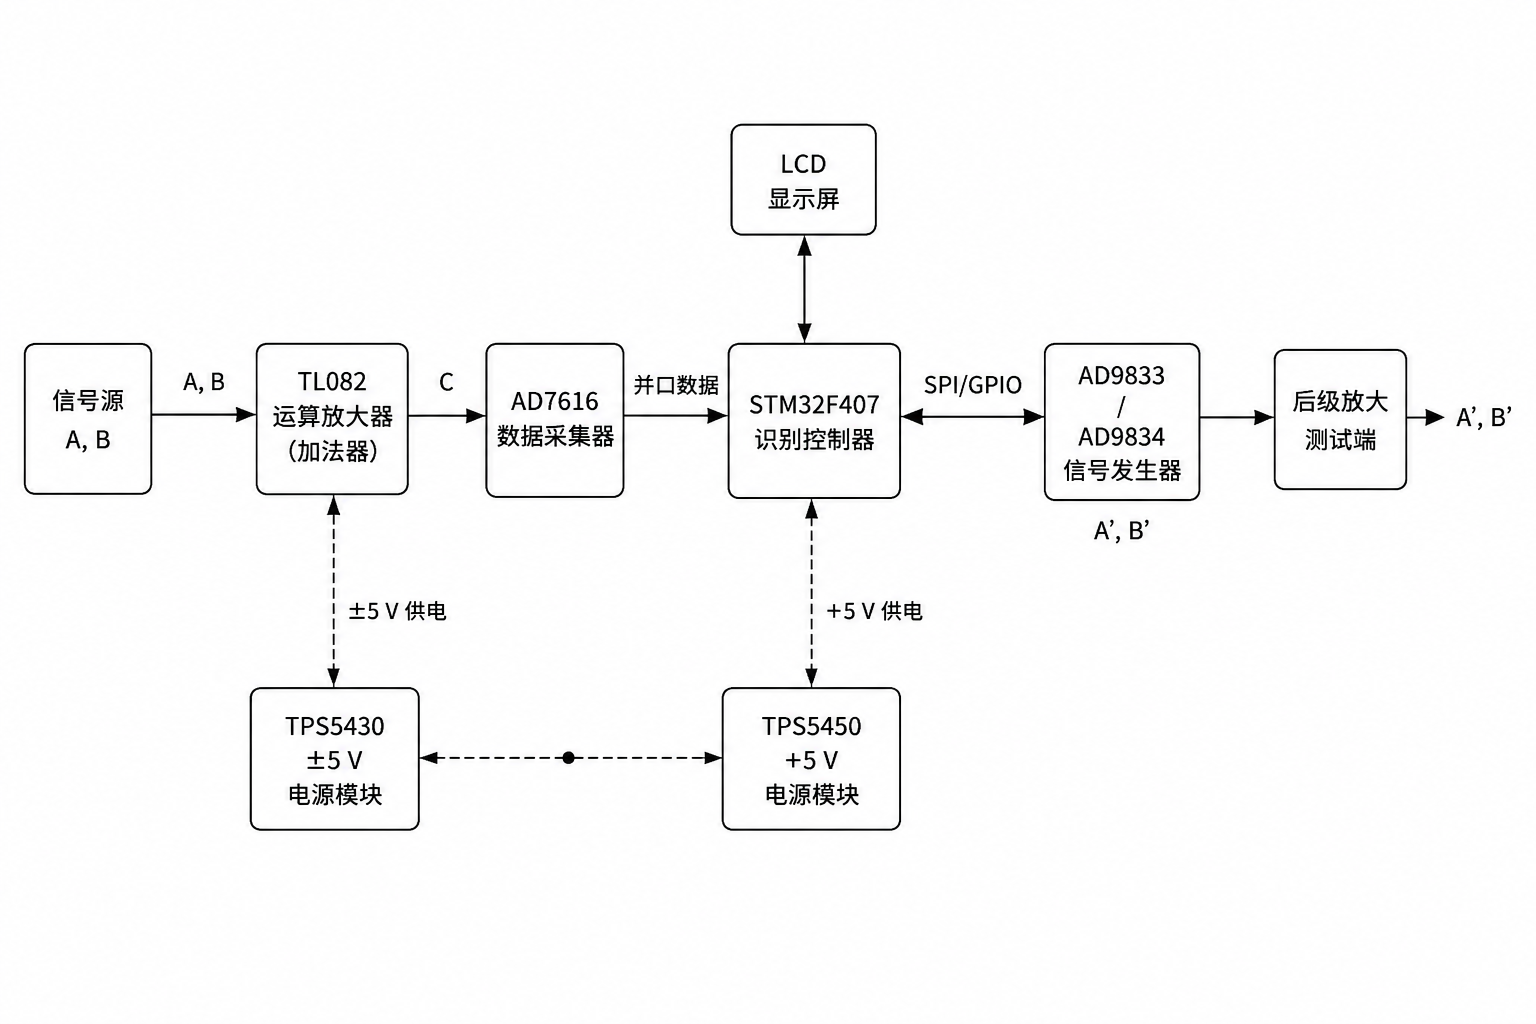
\includegraphics[width=\textwidth]{图一.png}
\caption{本设计实际系统框图}
\label{fig:system_block}
\end{figure}

\section{理论分析与计算}

\subsection{信号模型}

加法器输出为
\begin{equation}
  C(t)=A(t)+B(t).
\end{equation}
当 $A(t)$、$B(t)$ 为不同频率的正弦波时，频谱中会出现两个主谱峰：
\begin{equation}
  A(t)=\frac{V_{pp}}{2}\sin(2\pi f_A t+\phi_A),\quad
  B(t)=\frac{V_{pp}}{2}\sin(2\pi f_B t+\phi_B).
\end{equation}
由于题目规定 $f_A<f_B$，识别后将低频分量映射为 $A'$，高频分量映射为 $B'$。

三角波可展开为奇次谐波级数：
\begin{equation}
  x_{\triangle}(t)=\frac{8A}{\pi^2}\sum_{m=0}^{\infty}\frac{(-1)^m}{(2m+1)^2}
  \sin\left((2m+1)\omega t\right).
\end{equation}
因此三角波的三次谐波幅度约为基波的 $1/9$，五次谐波约为基波的 $1/25$。程序中利用三次、五次谐波相对幅度对正弦波和三角波进行判别。

\subsection{采样率与 FFT 分辨率}

AD7616 最高采样率为 1 MSPS，本设计取
\begin{equation}
  f_s=500\text{ kSPS}.
\end{equation}
最高输入基波为 100 kHz，满足奈奎斯特采样条件 $f_s>2f_{\max}$。程序每帧采集 $N=2048$ 点，FFT 频率分辨率为
\begin{equation}
  \Delta f=\frac{f_s}{N}=\frac{500000}{2048}\approx244.14\text{ Hz}.
\end{equation}
该分辨率足以区分 5 kHz 或 10 kHz 的题目频率栅格。为降低频谱泄漏，采样数据先去直流均值并乘 Hann 窗：
\begin{equation}
  w[n]=0.5-0.5\cos\left(\frac{2\pi n}{N-1}\right).
\end{equation}
谱峰位置使用抛物线插值修正，以提高频率估计精度。

\subsection{频率栅格吸附}

FFT 估计值存在窗函数、有限采样长度和输入噪声带来的误差。题目频率为 10 kHz 或 5 kHz 整数倍，因此在识别场景后将估计频率吸附到最近栅格：
\begin{equation}
  \hat f_{\text{grid}}=\operatorname{round}\left(\frac{\hat f}{f_g}\right)f_g,
\end{equation}
其中基本项 $f_g=10\text{ kHz}$，发挥项 $f_g=5\text{ kHz}$。若估计值与栅格点距离小于设定容差，则采用栅格频率作为 DDS 输出频率。这样可避免 FFT 估计误差导致示波器上 $A'$、$B'$ 与原信号缓慢漂移。

\subsection{DDS 频率控制字}

AD9833 和 AD9834 均采用 28 位频率控制字。DDS 输出频率满足
\begin{equation}
  f_{\text{out}}=\frac{M f_{\text{clk}}}{2^{28}},
\end{equation}
其中 $M$ 为频率控制字。故
\begin{equation}
  M=\operatorname{round}\left(\frac{f_{\text{out}}2^{28}}{f_{\text{clk}}}\right).
\end{equation}
AD9833 模块主频为 25 MHz，则频率分辨率约为
\begin{equation}
  \Delta f_{\text{AD9833}}=\frac{25\text{ MHz}}{2^{28}}\approx0.093\text{ Hz}.
\end{equation}
AD9834 模块程序中按 75 MHz 主频计算，则频率分辨率约为
\begin{equation}
  \Delta f_{\text{AD9834}}=\frac{75\text{ MHz}}{2^{28}}\approx0.279\text{ Hz}.
\end{equation}
两者均远小于题目频率栅格间隔，能够保证同频稳定输出。

\subsection{相位与移相说明}

FFT 可通过
\begin{equation}
  \phi_k=\operatorname{atan2}(X_i[k],X_r[k])
\end{equation}
估计谱峰相位。若后续测试需要 $A'$、$B'$ 与原信号保持固定相位关系，可将相位换算为 DDS 相位字：
\begin{equation}
  P=\operatorname{round}\left(\frac{\phi}{2\pi}\cdot 4096\right).
\end{equation}
当前程序以同频稳定显示为主要目标，DDS 输出相位固定。示波器触发观测时，只要输出频率与原信号一致，相对相位为常数，即可满足稳定不漂移的测试要求。

\section{电路设计}

\subsection{加法器}

加法器为独立电路板，与分离电路只连接混合信号 $C$ 和地线。核心器件为一片 TL082 双运放（U1），其中 U1.1 构成反相求和放大器：输入 $A$、$B$ 分别经 SMA 连接器接入，通过 10 k$\Omega$ 输入电阻送入反相端，反馈电阻为 2 k$\Omega$，同相端经电阻接地。输入端并联 DSK14 钳位二极管（D3、D4）进行过压保护。U1.2 为第二路运放，经 0 $\Omega$ 跳线连接至输出 SMA 端。图 \ref{fig:adder} 为加法器原理示意。反相求和结构使输出整体反相，不影响频率识别与后续 DDS 重构。

\begin{figure}[H]
\centering
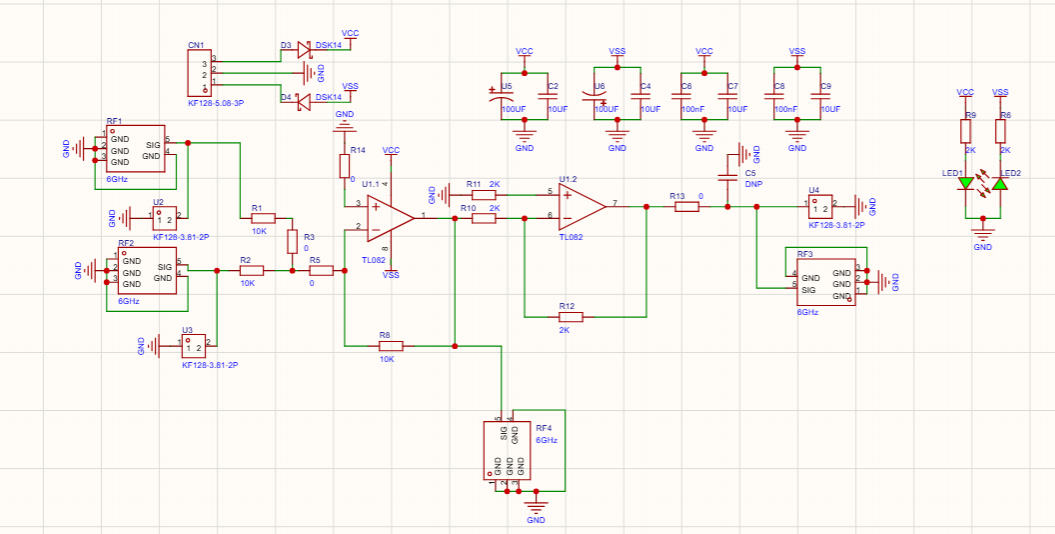
\includegraphics[width=\textwidth]{图二.png}
\caption{独立加法器原理示意}
\label{fig:adder}
\end{figure}

\noindent\textbf{供电说明：}
TPS5430 产生正负电源为 TL082 加法器运放供电。TPS5450 提供系统正 5 V，用于 STM32F407 主控、DDS 模块、LCD 背光及后级 OPA177 放大模块，并可经后级稳压获得数字 3.3 V。

\subsection{采集电路}

AD7616 配置为并口模式，数据线 DB0--DB15 接 STM32F407 的 PD0--PD15。控制线包括 CS、RD、WR、RST、BUSY、CONVST、RNG0、RNG1 和通道选择线。CONVST 由 TIM2 的 PWM 输出产生采样节拍，BUSY 下降后读取 GPIOD 输入寄存器。

\begin{table}[H]
\centering
\caption{AD7616 与 STM32F407 主要连接}
\begin{tabular*}{\textwidth}{@{\extracolsep{\fill}}lll@{}}
\toprule
AD7616 信号 & STM32F407 引脚 & 说明 \\
\midrule
DB0--DB15 & PD0--PD15 & 16 位并行数据总线 \\
CONVST & PA15/TIM2\_CH1 & 采样触发 \\
BUSY & PA11 & 转换忙信号 \\
CS/RD/WR/RST & PC6/PC7/PC8/PC9 & 并口读写与复位控制 \\
RNG0/RNG1 & PC10/PC11 & 输入量程选择 \\
CHS0--CHS2 & PC12/PA8/PA9 & 通道选择 \\
SER/PAR & PA10 & 并口/串口模式选择 \\
\bottomrule
\end{tabular*}
\end{table}

\subsection{DDS 输出电路}

输出端采用两片独立 DDS。AD9833 负责低频分量 $A'$，AD9834 负责高频分量 $B'$。两片 DDS 均使用 GPIO 模拟 SPI 写入 16 位控制字，互不共用片选和数据线。DDS 原始输出再接后级放大模块，调整幅度到不小于 1 Vpp，并提供 $A'$、$B'$ 测试端。后级放大电路如图 \ref{fig:output_amp} 所示，采用 OPA177 精密运放，由 TPS5450 提供 +5 V 供电。输入端经 0.1 $\mu$F 电容（C4）交流耦合，通过 5 $\Omega$ 电阻（R1）接入运放同相输入端，同相端并联 10 k$\Omega$ 电阻接地提供偏置；反馈通路采用 100 k$\Omega$ 电阻（R2），输出端经 0.1 $\mu$F 电容（C2）交流耦合后送出。OPA177 的高精度、低失调特性有利于保持 DDS 输出波形的保真度。

\begin{table}[H]
\centering
\caption{DDS 输出连接}
\begin{tabular*}{\textwidth}{@{\extracolsep{\fill}}llll@{}}
\toprule
通道 & 器件 & STM32 控制线 & 输出用途 \\
\midrule
$A'$ & AD9833 & PA2/PA4/PA6 & 低频分量，正弦/三角输出 \\
$B'$ & AD9834 & PE2--PE6、PC0 & 高频分量，正弦/三角输出 \\
\bottomrule
\end{tabular*}
\end{table}

\begin{figure}[H]
\centering
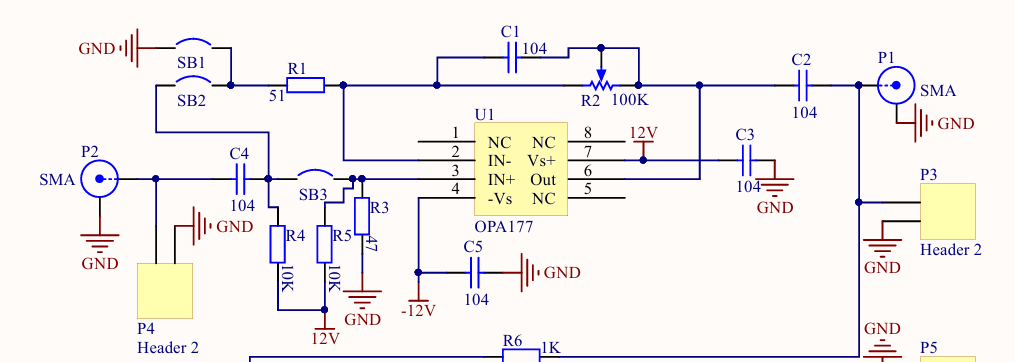
\includegraphics[width=\textwidth]{图三.png}
\caption{后级放大模块原理示意}
\label{fig:output_amp}
\end{figure}

\section{程序设计}

\subsection{软件总体流程}

程序采用状态机结构，上电后自动初始化 AD7616、DDS、LCD 和定时器，然后按“采集、FFT、识别、DDS 输出、LCD 显示”的顺序循环工作。若当前帧无法给出有效识别结果，则重新采集并再次分析。

\subsection{采样驱动}

TIM2 工作在 PWM 模式，周期为 167，APB1 定时器时钟为 84 MHz，因此采样触发频率为
\begin{equation}
  f_s=\frac{84\text{ MHz}}{167+1}=500\text{ kHz}.
\end{equation}
定时器更新中断中首先轮询 AD7616 的 BUSY 引脚，设置 20 次轮询超时上限；若 BUSY 在超时内拉低，则拉低 CS/RD，直接读取 GPIOD$\to$IDR 的 16 位数据，随后拉高 RD/CS 完成一次采样。若 BUSY 超时未拉低，中断置位采集错误标志并终止当前帧。与逐位调用 HAL\_GPIO\_ReadPin 相比，寄存器读法显著降低采样开销，保证 500 kSPS 下能完成每点读取。当 2048 点全部填满后置位帧完成标志，主循环检测到该标志后停止 TIM2 并切换至分析状态。

\subsection{频谱识别算法}

DSP 模块的输入为 2048 点有符号采样数据。处理步骤如下：
\begin{enumerate}
  \item 计算均值并去除直流分量。
  \item 对时域数据乘 Hann 窗，降低非整周期采样导致的旁瓣泄漏。
  \item 调用 CMSIS-DSP 的 2048 点复数 FFT，得到幅度谱。
  \item 在 20 kHz--100 kHz 范围内寻找最大谱峰作为主峰。为避免噪声尖峰被误判，在主峰位置左右各保留 3 个 bin 的保护带，排除该区域后在同范围内寻找次大谱峰作为次峰。
  \item 次峰的有效性判定条件为：次峰幅度不低于主峰幅度的 5\%，否则认为输入为单频信号，不进行双信号分离。
  \item 对主峰和次峰分别做抛物线插值，估计更精确的频率。
  \item 对每个分量搜索三次和五次谐波，用于判别正弦波或三角波。在搜索谐波时，若某次谐波的幅度超过基波幅度的 50\%，则判定该谱峰为另一路独立信号而非真正的谐波分量，避免将双信号误判为单信号的谐波。
  \item 三角波的 3 次和 5 次谐波折叠后可能相互重叠，当低频分量的 5 次谐波幅度与高频分量的 5 次谐波折叠到相同频率且低频分量的 5 次谐波比率低于 7.5\% 时，将低频分量从三角波修正为正弦波，避免误分类。
  \item 根据低频为 $A$、高频为 $B$ 的规则生成输出计划。
\end{enumerate}

由于三角波高次谐波可能超过奈奎斯特频率，程序对谐波频率进行折叠搜索：
\begin{equation}
  f_{\text{fold}} =
  \begin{cases}
    f_h \bmod f_s, & f_h \bmod f_s \leq f_s/2,\\
    f_s-(f_h \bmod f_s), & f_h \bmod f_s > f_s/2.
  \end{cases}
\end{equation}
这样在 500 kSPS 采样率下仍能利用部分折叠谐波辅助识别高频三角波。

\subsection{DDS 控制}

输出模块将识别到的波形类型映射为 DDS 控制字。正弦波使用 DDS 正弦输出模式，三角波使用三角输出模式。AD9833 使用频率寄存器 FREQ0 输出 $A'$，AD9834 使用 FREQ0 输出 $B'$。每次更新前先置 RESET，再写入频率控制字，最后选择波形并退出 RESET，以减少频率切换时的输出毛刺。

为提高不同测试场景下的识别成功率，程序对识别结果进行场景分类。对于基本项，当两路信号分别接近 50 kHz 和 100 kHz 时直接锁定为固定频率；对于发挥部分，若两路信号均为正弦波且均为 10 kHz 整数倍，则将估计频率吸附到 10 kHz 栅格，若为正弦/三角波混合且均为 5 kHz 整数倍，则吸附到 5 kHz 栅格。吸附算法为
\begin{equation}
  \hat{f}_{\text{grid}}=\operatorname{round}\left(\frac{\hat{f}}{f_g}\right)f_g,
\end{equation}
其中基本项 $f_g=10\text{ kHz}$，发挥项 $f_g=5\text{ kHz}$。为防止错误吸附，设定容差为 800 Hz，若估计值与最近栅格点的距离超过该容差则保持原值不变。若 20 秒内未能识别出有效信号，系统报错并等待下一轮采集。

\section{测试方案与结果记录}

实际测试时使用双路函数信号源提供 $A$、$B$，示波器同时观察 $A$、$B$、$C$、$A'$、$B'$，并记录 LCD 显示值。测试步骤如下：
\begin{enumerate}
  \item 检查加法器供电和输出，确认 $C$ 幅度及频谱包含两路输入分量。
  \item 启动分离电路，观察 $A'$、$B'$ 是否稳定输出。
  \item 将示波器触发源设为 $A$，观察 $A'$ 是否同频稳定；再以 $B$ 为触发源观察 $B'$。
  \item 对基本项、10 kHz 栅格项和 5 kHz 栅格正弦/三角组合分别测试。
\end{enumerate}

\begin{table}[H]
\centering
\caption{测试记录表}
\scriptsize
\begin{tabular*}{\textwidth}{@{\extracolsep{\fill}}p{0.6cm}p{1.7cm}p{1.8cm}p{3.0cm}p{3.0cm}p{2.3cm}@{}}
\toprule
序号 & 输入 $A$ & 输入 $B$ & LCD 识别结果 & DDS 输出 & 示波器结论 \\
\midrule
1 & 50 kHz 正弦 & 100 kHz 正弦 & A:50 kHz 正弦；B:100 kHz 正弦 & $A'$:50 kHz 正弦；$B'$:100 kHz 正弦 & 同频稳定，无明显失真 \\
2 & 30 kHz 正弦 & 80 kHz 正弦 & A:30 kHz 正弦；B:80 kHz 正弦 & $A'$:30 kHz 正弦；$B'$:80 kHz 正弦 & 同频稳定，无明显失真 \\
3 & 25 kHz 三角 & 70 kHz 正弦 & A:25 kHz 三角；B:70 kHz 正弦 & $A'$:25 kHz 三角；$B'$:70 kHz 正弦 & 同频稳定，无明显失真 \\
4 & 40 kHz 正弦 & 95 kHz 三角 & A:40 kHz 正弦；B:95 kHz 三角 & $A'$:40 kHz 正弦；$B'$:95 kHz 三角 & 同频稳定，无明显失真 \\
\bottomrule
\end{tabular*}
\end{table}

从理论分辨率看，FFT 频率 bin 间隔约为 244 Hz，远小于题目的 5 kHz 最小频率栅格。DDS 频率分辨率低于 1 Hz，频率重构误差远小于 FFT 识别误差。

\section{改进方案}

本设计当前主控为 STM32F407，主频 168 MHz，已能完成 500 kSPS、2048 点 FFT 和双 DDS 控制。后续可从以下方向改进：
\begin{itemize}
  \item 增加相位估计与 DDS 相位字输出，使 $A'$、$B'$ 与原信号保持可控相位差。当前 DDS 输出相位固定，若测试要求输出与输入保持特定相位关系，可通过 FFT 估计各分量初相并写入 AD9833/AD9834 的相位寄存器实现。
  \item 增加可编程增益放大模块，例如采用 AD8367 可变增益放大器。当前后级放大增益固定，面对不同幅度的输入信号时适应性有限；引入程控增益后，可根据采样信号幅度自动调整放大倍数，使 DDS 输出幅度始终满足不小于 1 Vpp 的要求。
  \item 增加多帧平均和置信度判断，提高低信噪比下的识别稳定性。
  \item 将 LCD 频谱显示做成实时柱状谱，便于测试时直观看到分离依据。
\end{itemize}

\section{结论}

本设计采用 AD7616 高速采样、STM32F407 频谱识别和 AD9833/AD9834 双 DDS 重构的数字分离方案。与固定模拟滤波器相比，该方案能适应题目中不同频点和正弦/三角波组合；与 AD9854 方案相比，硬件与程序复杂度更低，更符合本题 20--100 kHz、1 Vpp 输出的需求。通过 500 kSPS 采样、2048 点 FFT、谐波波形判别和频率栅格吸附，系统能够在理论上满足自动分离与同频稳定输出的要求。

\end{document}
